
\chapter{Исследование модельного порыва}


В прямых трубах круглого сечения, как и в некоторых других сдвиговых течениях, переход к турбулентности может происходить без потери ламинарным течением линейной устойчивости. В частности, в приведенной в разделе \ref{math_section} постановке ламинарное течение (течение Пуазейля в круглой трубе) линейно устойчиво при всех числах Рейнольдса \cite{Kerswell2005}. Для выхода на турбулентный режим течения необходимо внести в поток возмущения достаточно большой амплитуды, в то время как малые возмущения ламинарного течения затухают. В таких условиях существуют возмущения некоторой критической амплитуды, отделяющие возмущения, вызывающие переход к турбулентности, от затухающих. В фазовом пространстве соответствующие критическим возмущениям решения принадлежат сепаратрисе, отделяющей области притяжения решений, соответствующих ламинарному и турбулентному режимам течения. Принадлежащее в первый момент времени сепаратрисе решение остается на сепаратрисе. Хотя решение, эволюционирующее на сепаратрисе, неустойчиво и не может наблюдаться в эксперименте, оно может быть получено численно. Замечено, что решение на сепаратрисе сохраняет некоторое характерные черты турбулентного течения, но при этом имеет более простую форму и динамику. 

Метод поиска решения на сепаратрисе предложен в работе \cite{Skufca2006}. Первые расчеты решения на сепаратрисе в круглой трубе выполнены в расчетной области небольшой протяженности (с условием периодичности вдоль потока) \cite{Schneider2007}. В расчетах \cite{Mellibovsky2009transition, Duguet2010}, выполненных в протяженной расчетной области, обнаружено, что при переходных числах Рейнольдса решение на сепаратрисе в круглой трубе имеет пространственно локализованную структуру. При этом, если турбулентность существует в форме пространственно локализованных порывов до $\Re \approx 2700$, решение на сепаратрисе имеет локализованную структуру по крайней мере до $\Re = 6000$. С ростом числа Рейнольдса амплитуда отклонения от ламинарного течения и протяженность области локализации в решении на сепаратрисе снижаются \cite{Duguet2010}, что дает основание полагать, что решение на сепаратрисе сохраняет локализованную структуру и при больших числах Рейнольдса. Как отмечено в \cite{Duguet2010, Avila2013}, решение на сепаратрисе в круглой трубе воспроизводит ряд характерных особенностей турбулентного порыва, и при небольших значениях числа Рейнольдса их характеристики оказываются близки друг к другу. Структуры, напоминающие локализованное решение на сепаратрисе, наблюдались в экспериментах \cite{deLozar2012} и в численных расчетах \cite{Manneville2011} при затухании турбулентного течения. 
% Расчеты решения на сепаратрисе в плоском течении Куэтта \cite{Schneider2008}
% Решение на сепаратрисе в плоском течении Куэтта в протяженной расчетной области имеет локализованную структуру \cite{Duguet2009}

В работе \cite{Avila2013} обнаружено, что при наложении на решение, описывающее течение в круглой трубе, дополнительных условий симметрии при переходном значении числа Рейнольдса решение, эволюционирующее на сепаратрисе, приближается к условно периодическому решению. Предельное решение сохраняет пространственно локализованную структуру, но в сопутствующей системе отсчета оказывается периодическим по времени. Помимо пространственной локализации предельное решение воспроизводит некоторые другие характерные особенности турбулентного порыва. Мы будем называть это решение {\it модельным порывом}. Простота поведения модельного порыва позволяет выполнить его подробное исследование, что может помочь прояснить свойства турбулентного порыва. 

В главе представлен метод получения модельного порыва, описаны его основные характеристики и внутренняя структура; даны оценки достоверности полученных результатов. Детальное описание внутренней структуры модельного порыва выполнено автором диссертации и является новым научным результатом. Основные результаты, приведенные в этом разделе, опубликованы в работах автора диссертации \cite{MZG2015, Kazan2015, KMU2015}. 


\section{Получение модельного порыва} \label{edge_seq}

Следуя \cite{Avila2013}, решение поставленной в разделе \ref{math_section} задачи ищется с дополнительными ограничениями диаметральной симметричности и $\pi$-периодичности в угловом направлении:
\begin{equation}\label{sym_eq}
(v_x, v_r, v_\theta)(x, r, -\theta, t) = (v_x, v_r, -v_\theta)(x, r, \theta, t),
\end{equation}
\begin{equation}\label{per_eq}
(v_x, v_r, v_\theta)(x, r, \theta+\pi, t) = (v_x, v_r, v_\theta)(x, r, \theta, t).
\end{equation}
Здесь $(x, r, \theta)$ --- цилиндрические координаты, $(v_x, v_r, v_\theta)$ --- продольная, радиальная и угловая компоненты вектора скорости. Наложение ограничений \eqref{sym_eq}, \eqref{per_eq} упрощает поведение решения в пространстве, делает его более определенным. Условие \eqref{sym_eq} ограничивает возможность смещения турбулентных структур в угловом направлении.  Турбулентные порывы, рассчитанные при $Re=2000$ с учетом и без учета условий \eqref{sym_eq}, \eqref{per_eq} изображены на рисунке~\ref{3D_img} (представлены области пониженной и повышенной на $0.1$ скорости относительно течения Пуазейля). В обоих случаях порыв имеет центральное ядро с пониженной скоростью и систему вытянутых вдоль стенки трубы, чередующихся в угловом направлении полос замедления и ускорения. На симметричном порыве полосы гораздо более структурированы. Их угловое положение не меняется в процессе эволюции: угловые области $\theta=k\pi/2$, $k$ от $0$ до $3$, где в силу \eqref{sym_eq}, \eqref{per_eq} угловая компонента скорости тождественно равна нулю, заняты полосами ускорения, промежуточные области $\theta=\pi/4+k\pi/2$ --- полосами замедления. На порыве без условий симметрии наблюдаются значительные по амплитуде случайные по пространственному расположению флуктуации, разрывающие сплошность полосчатых структур. На симметричном порыве тоже заметна флуктуирующая компонента, которая в этом случае выглядит гораздо более регулярной. Отметим, что несмотря на заметную пространственную регулярность, временн\'{о}е поведение симметричного порыва остается хаотичным.


\begin{figure}[h]
\center{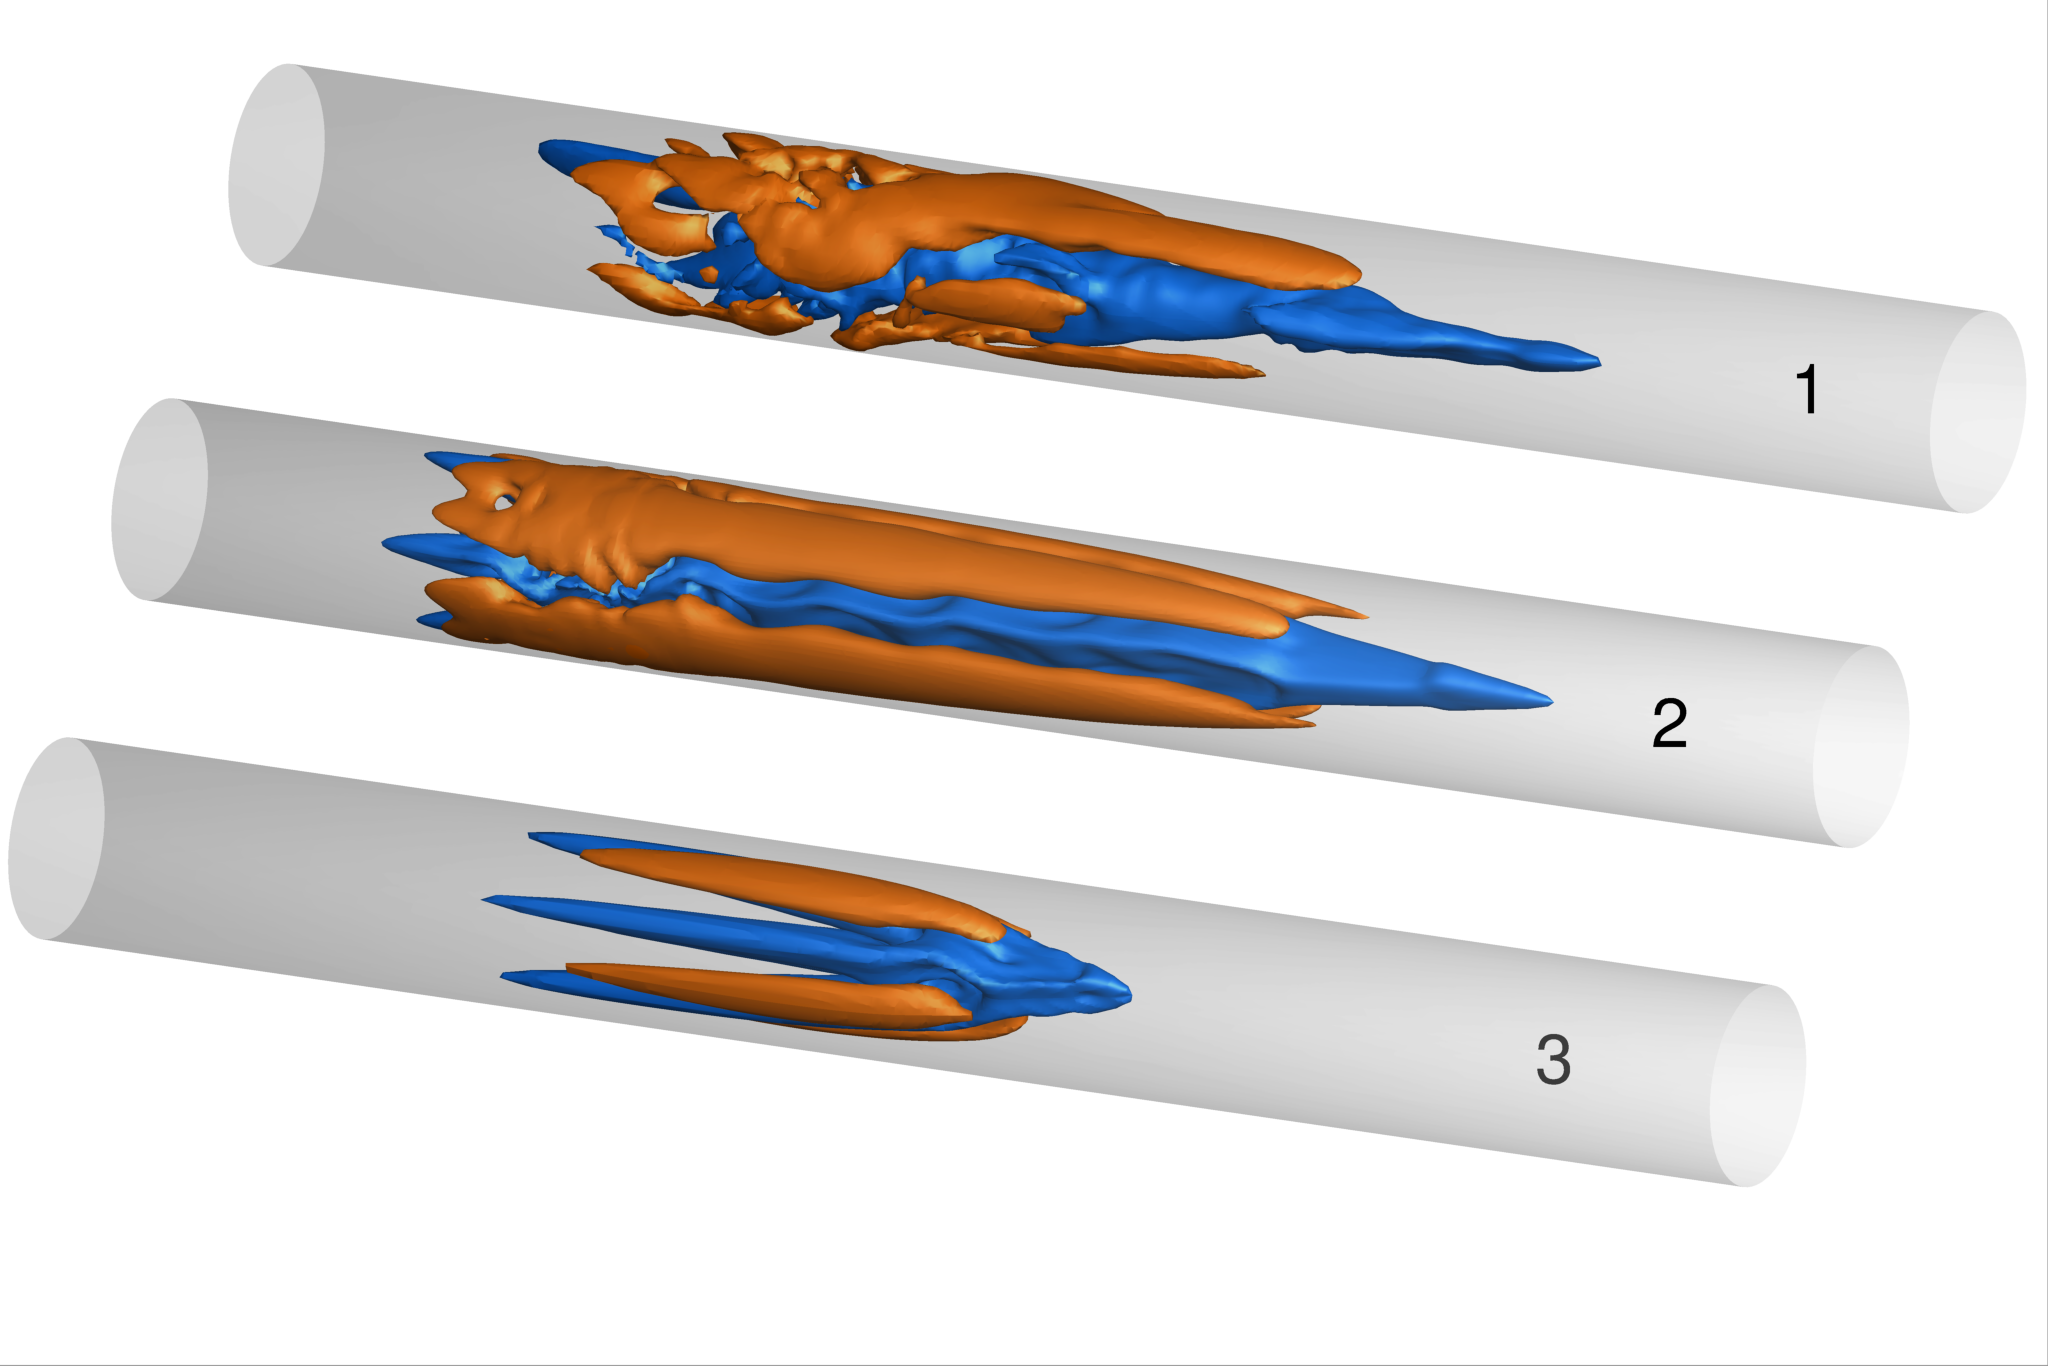
\includegraphics[width=1\linewidth]{3D_cmp.png}}
\caption{Визуализация численных расчетов турбулентных порывов: 1 --- $\Re = 2000$; 2 --- $\Re = 2000$ с учетом \eqref{sym_eq}, \eqref{per_eq}; 3 --- решение на сепаратрисе, $\Re = 2200$. Темным и светлым тоном выделены поверхности скорости $-0.1$ и $+0.1$ относительно скорости течения Пуазейля. Поток направлен слева направо.}
\label{3D_img}
\end{figure}

Предельное решение на сепаратрисе получено при $Re=2200$. Условие \eqref{per_eq} при \eqref{sym_eq} порождает условие отражения относительно сечения $\theta = \pi/2$, аналогичное условию отражения относительно сечения $\theta = 0$:
\begin{equation} \label{sym2_eq}
(v_x, v_r, v_\theta)(x, r, \pi/2 + \theta, t) = (v_x, v_r, -v_\theta)(x, r, \pi / 2 - \theta, t).
\end{equation}
С учетом \eqref{sym_eq}, \eqref{sym2_eq} расчет проводился для четверти объема трубы $0\leqslant\theta\leqslant\pi/2$. Исходное решение найдено при $L_x = 80$ на сетке, содержащей $512 \times 32 \times  32$ ячеек в продольном, радиальном и угловом направлениях. 

Предварительно найденное турбулентное решение $\v_{turb}(\x,t)$ используется в итерационной процедуре отыскания предельного решения на сепаратрисе. Задача решается с начальным условием
\begin{equation} \label{edge_init_eq}
\v(\x,t=0) = \v_{Pois}(\x)+\alpha(\v_{turb}(\x,t=t_0) - \v_{Pois}(\x)).
\end{equation}
Здесь $\v_{Pois}=(1-r^2,0,0)$ --- течение Пуазейля, $t_0$ --- некоторый фиксированный момент времени, $\alpha \in [0,1]$ --- скалярный параметр. Значение $\alpha=0$ соответствует нулевому возмущению, и решением при $t > 0$ остается течение Пуазейля. Выбирая $\alpha=1$, уже в начальный момент времени реализуется турбулентный режим, который сохраняется при $t > 0$. При промежуточных значениях $\alpha$ происходит стремление решения либо к одному, либо к другому режиму. Применяя метод деления пополам, мы постепенно отыскиваем то значение $\alpha$, при котором решение эволюционирует на сепаратрисе, разделяющей области притяжения двух режимов течения. Суть метода состоит в том, что если при текущем значении $\alpha$ трехмерные возмущения затухают, на новой итерации $\alpha$ увеличивается; если развивается турбулентный режим течения, $\alpha$ уменьшается. На рисунке \ref{bisection_pic} представлены графики $A(t)$ – среднеквадратичного по всему объему отклонения поля скорости от течения Пуазейля для нескольких значений $\alpha$, демонстрирующие сходимость итерационного процесса. При уточнении значения $\alpha$ продлевается длительность балансирования решения на сепаратрисе.


\begin{figure}
\center{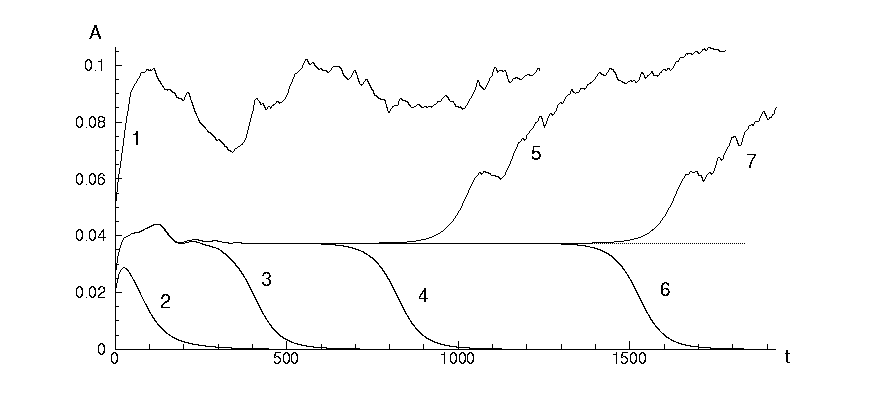
\includegraphics[width=1\linewidth]{bisection.png}}
\caption{Итерационный процесс построения решения на сепаратрисе. 1--7 --- эволюция среднеквадратичной амплитуды возмущений $A(t)$ при уточнении значения $\alpha$.}
\label{bisection_pic}
\end{figure}

С каждой новой итерацией решение проводит на сепаратрисе в среднем на 30 единиц времени больше. В расчетах для представления действительных числе были применены 64-битные числа с плавающей запятой. В этом случае может быть выполнено до 50 итераций метода поиска решения на сепаратрисе. Соответственно, решение можно удержать на сепаратрисе в течении приблизительно 1500 единиц времени. Из них ориентировочно первые 500 единиц происходит перестройка решения, после чего режим течения устанавливается. В согласии с результатами \cite{Avila2013}, решение на сепаратрисе при $\Re=2200$ постепенно выходит на условно периодический режим. Это решение, как и турбулентный порыв, имеет форму локализованной в пространстве структуры, которая сносится вниз по потоку с постоянной скоростью. В подвижной системе отсчета поле скорости в каждой точке испытывает периодические колебания. Для скорости сноса и периода колебаний получены значения $c_m=0.69$ и $T=60$ (в \cite{Avila2013} сообщается о $c_m=0.76$ и $T=60$). Во всех выполненных расчетах режим течения, устанавливающийся на сепаратрисе, не зависит от исходного турбулентного поля скорости $\v_{turb}$. 

Так как скорость сноса модельного порыва заранее не известна, решение на сепаратрисе было найдено в системе отсчета, двигающейся со скоростью $0.5$. После того, как решение на сепаратрисе найдено, изменить скорость перемещения системы отсчета уже не представляется возможным вследствие высокой чувствительности решения к возмущениям, возникающим в данном случае в результате неточностей численного интегрирования. Чтобы получить решение в сопутствующей системе отсчета, метод поиска решения на сепаратрисе применен повторно в системе отсчета, двигающейся с уже известной скоростью перемещения порыва. 

Сравнение предельного решения на сепаратрисе с турбулентным порывом, представленное на рисунке \ref{3D_img}, показывает качественное согласие этих решений. Во всех структурах имеются протяженные области ускоренного и замедленного движения, концентрирующиеся в пристенной области трубы. Сохраняется и основная качественная особенность порыва --- медленное понижение осевой скорости на переднем фронте и более резкое её восстановление на заднем (смотри рисунок \ref{ucl_cmp_img}). Мы будем называть предельное решение на сепаратрисе {\it модельным порывом}.  

\begin{figure}
\center{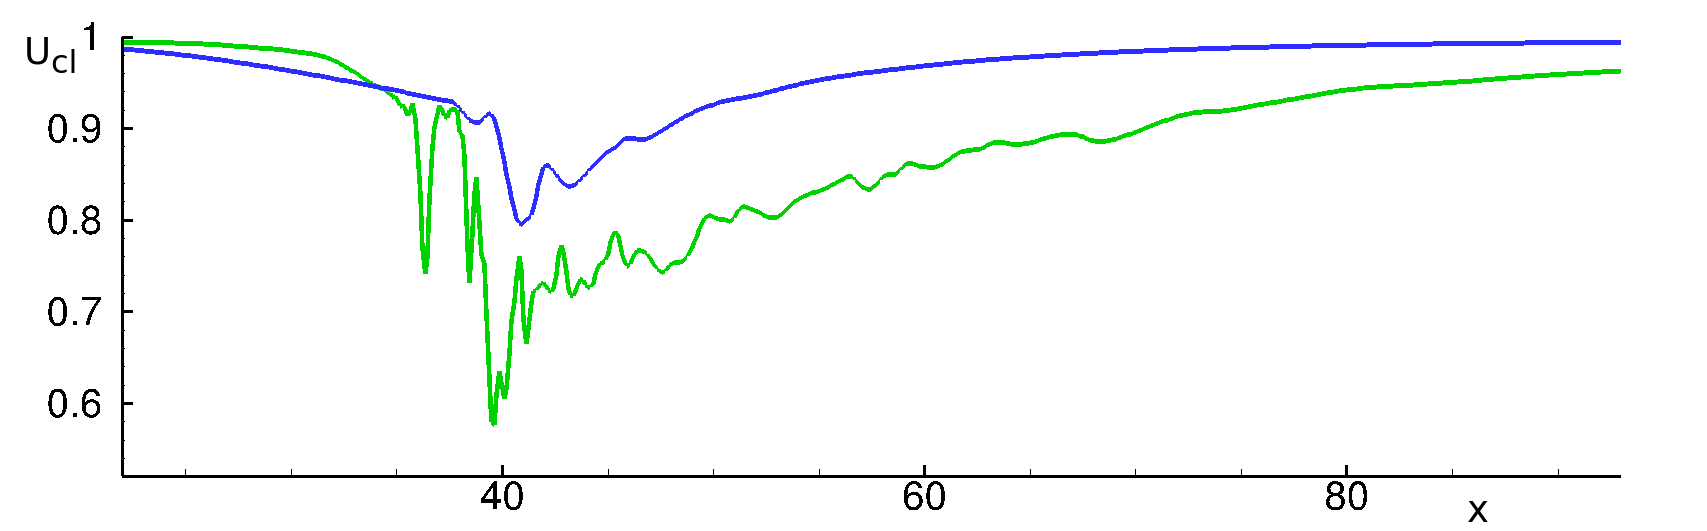
\includegraphics[width=0.7\linewidth]{ucl_cmp.png}}
\caption{Сравнение скорости на оси трубы в турбулентном (1) и модельном (2) порывах.}
\label{ucl_cmp_img}
\end{figure}

Для того, чтобы установить влияние условия периодичности вдоль трубы на предельное решение, решение было найдено в расчетной области вдвое большей протяженности, при $L_x = 160$ (число узлов сетки в продольном направлении также удвоено). Также при исходном значении $L_x = 80$ решение было получено на более подробной сетке, содержащей $1024 \times 64 \times 64$ ячеек (в сравнении с исходной сеткой в каждом направлении число ячеек удвоено). Результаты, полученные на трех сетках, качественно совпадают и количественно близки. Для сравнения, на рисунке \ref{amp_pic} представлены некоторые интегральные характеристики модельного порыва, полученные на различных сетках (подробное описание изображенных величин приведено в следующем разделе). Полученные результаты подтверждают достаточность расчетной сетки и длины расчетной области для адекватного воспроизведения модельного порыва, а также то, что его пространственная локализация не связана с условием периодичности вдоль трубы. Характеристики полученного модельного порыва согласуются с результатами работы \cite{Avila2013}. Это подтверждает, что найденное решение является решением математической задачи и не зависит от численного метода, которым оно было найдено. В работе \cite{Avila2013} решение получено двумя методами --- полностью спектральным \cite{Meseguer2007} и спектрально-конечно-разностным \cite{Willis2009}. В нашем случае применен полностью конечно-разностный метод \cite{Nikitin2006}. Также, модельный порыв был воспроизведен в работе \cite{Chantry2014} спектрально-конечно-разностным методом \cite{Willis2009}; авторами также сообщается о совпадении результатов с \cite{Avila2013}. 


\section{Основные свойства модельного порыва}

При $\Re=2200$ модельный порыв имеет длину около $40R$ и перемещается вдоль трубы со скоростью $c_m = 0.69U$ (<<m>> --- <<model puff>>). В подвижной системе отсчета он является периодическим по времени с периодом $T = 60 R/U$. Характерным свойством модельного порыва является наличие вытянутых вдоль потока областей с повышенным и пониженным значением продольной компоненты скорости, чередующихся в угловом направлении (смотри рисунок \ref{3D_img}). Полосы повышенной скорости целиком расположены около стенки трубы, полосы замедления соединяются в единое целое в приосевой области вблизи переднего фронта. Наличие вытянутых вдоль потока полос ускоренного и замедленного движения --- характерное свойство любого пристенного турбулентного течения. Однако, в отличие от реальной турбулентности, где полосы случайно блуждают во времени и в пространстве, в рассматриваемом решении полосы сохраняют свое положение и форму, лишь слегка искажаясь периодическими колебаниями. 

\begin{figure}
\center{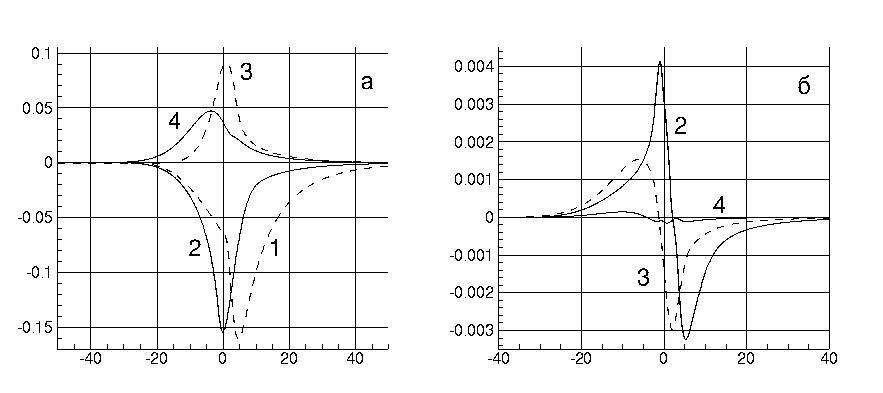
\includegraphics[width=1\linewidth]{U2D.png}}
\caption{Распределения вдоль трубы продольной (a) и радиальной (b) компоненты осесимметричной составляющей скорости $\V_{2D}$ для нескольких расстояний от оси трубы: 1–4 – r = 0, 0.4, 0.7, 0.9}
\label{U2D_pic}
\end{figure}

Для удобства перейдем в подвижную систему координат, перемещающуюся вдоль трубы со скоростью сноса локализованной структуры $c_m$. В подвижной системе решение представляется в виде суперпозиции стационарной составляющей $\V(\x) = \overline{\v}^t$ и колебательной $\v_n(t,\x) = \v - \V$. Стационарную составляющую, в свою очередь, представим в виде суперпозиции осесимметричной $\V_{2D}(\x) = \overline{\V}^{\theta}$ и трехмерной $\V_{3D}(\x) = \V - \V_{2D}$ составляющих. Распределения продольной компоненты осесимметричной составляющей скорости вдоль трубы $V_{x,2D}(x)$ для нескольких расстояний от оси трубы представлены на рисунке \ref{U2D_pic}(а) (даны отклонения от течения Пуазейля). Начало системы отсчета $x=0$ помещено в сечение, в котором среднее отклонение скорости от течения Пуазейля максимально. Голова структуры, где начинает проявляться отклонение осевой скорости, располагается на расстоянии $x \approx 45$. Хвостовая часть структуры на сепаратрисе очерчена не так четко, как в турбулентных порывах, где восстановление скорости происходит на отрезке длиной в $3-5$ радиусов трубы.  Падение скорости в приосевой области трубы компенсируется ускорением у стенки. Поведение радиальной компоненты $V_{r,2D}$, показанное на рисунке \ref{U2D_pic}(b) соответствует изменению осевой скорости --- в зоне замедления на оси происходит растекание жидкости к стенкам, $V_{r,2D}>0$, в передней части происходит обратный процесс и $V_{r,2D}<0$.

\begin{figure}
\center{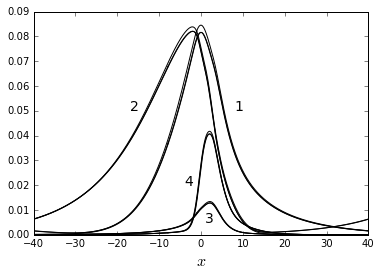
\includegraphics[width=0.6\linewidth]{amp.png}}
\caption{Распределения вдоль трубы среднеквадратичных по сечению амплитуд трех составляющих движения: 1 -- $\V_{2D}$ (отклонение от течения Пуазейля); 2, 3 -- продольная и поперечные компоненты скорости $\V_{3D}$; 4 -- $\v_{n}$. Представлены результаты, полученные на трех расчетных сетках, параметры которых приведены в разделе \ref{edge_seq}. Согласие результатов говорит об адекватности выбранных параметров сетки для расчета модельного порыва. }
\label{amp_pic}
\end{figure}

На рисунке \ref{amp_pic} приведены распределения по $x$ среднеквадратичных по сечению трубы амплитуд трех составляющих движения: стационарной осесимметричной (отклонение от течения Пуазейля) $A_{2D}$, стационарной трехмерной $A_{3D}$ и колебательной $A_n$. Распределение $A_{2D}(x)$ соответствует рисунку \ref{U2D_pic}. Отклонение от течения Пуазейля заметно на значительном отрезке от $x=-30$ до $x=40$. Максимум $A_{2D}$ составляет 8.4\%. Величина $A_{3D}$ характеризует интенсивность полосчатых структур. Как видно на рисунке~\ref{3D_img} полосчатые структуры появляются на некотором расстоянии вверх по потоку от головы порыва и сохраняются на значительном расстоянии позади него. В соответствии с этим $A_{3D}(x)$ имеет выраженную асимметрию относительно точки $x=-2$, где эта величина достигает максимума. Интенсивность полос быстро падает вниз по потоку и сохраняется на значительном расстоянии в верхней части потока. В отличие от стационарных полосчатых структур, колебательная составляющая движения сосредоточена на сравнительно непротяженном отрезке трубы от $x=-5$ до $x=15$ с максимальной амплитудой в 4\% при $x=2.5$.


\begin{figure}[h]
\center{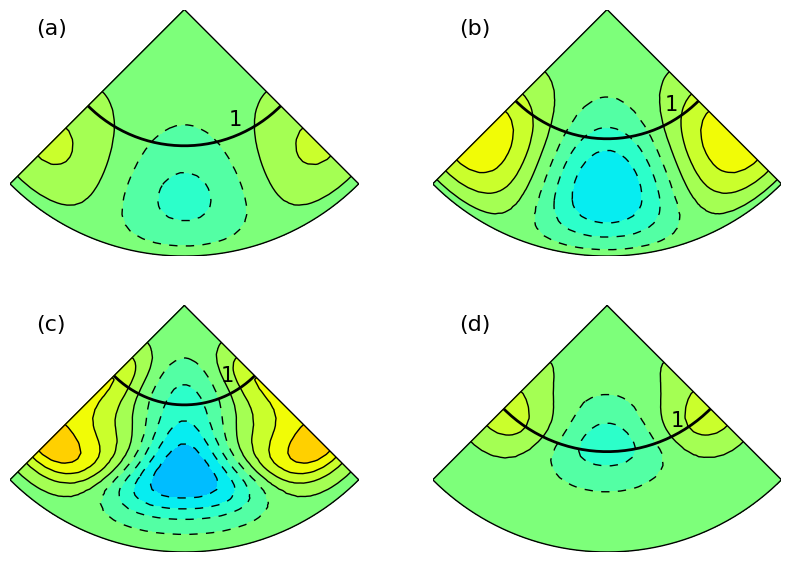
\includegraphics[width=0.8\linewidth]{V3D_cs.png}}
\caption{Распределения продольной составляющей $V_{x,3D}$ в нескольких сечениях трубы: (a)--(d) --- $x = -20, -10, 0, 5$. Сплошные изолинии --- положительная скорость, пунктирные изолинии --- отрицательная скорость, 1 --- линия, на которой относительная скорость жидкости равна нулю ($V_{x} = c_m$).}
\label{V3D_cs_pic}
\end{figure}


В трехмерную стационарную составляющую движения $V_{x,3D}$ попадают полосы повышенной и пониженной скорости. Поле $V_{x,3D}$ в нескольких сечениях трубы изображено на рисунке~\ref{V3D_cs_pic}. В каждом сечении трубы полосы пониженной скорости ($V_{x,3D} < 0$) проходят через центр расчетной области, при $\theta = \pi/4$. Полосы повышенной скорости ($V_{x,3D} > 0$) попадают на границы расчетной области в угловом направлении, находящиеся при $\theta = 0, \pi/2$. Среднее поле скорости оказывается симметрично относительно плоскости, проходящей через центр расчетной области при $\theta = \pi/4$, так как поле скорости решения на сепаратрисе $\v = (v_x, v_r, v_\theta)$ имеет дополнительную симметрию отражения относительно указанной плоскости со сдвигом на половину периода по времени:
\begin{equation}
(v_x, v_r, v_\theta)(x, r, \pi/4 + \theta, t) = (v_x, v_r, -v_\theta)(x, r, \pi/4 - \theta, t + T/2). 
\end{equation} 


\begin{figure}[h]
\center{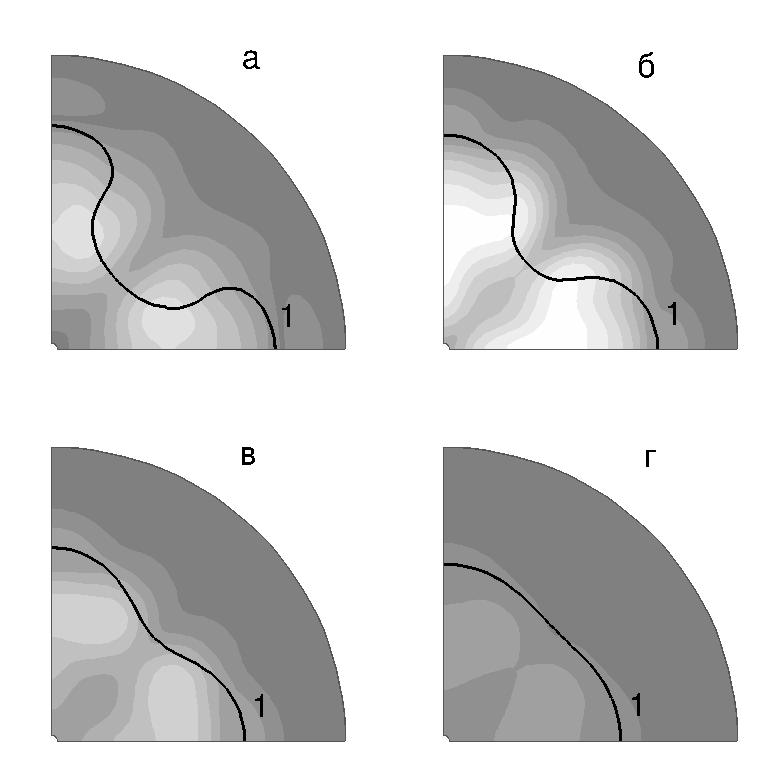
\includegraphics[width=0.8\linewidth]{puls_cs.png}}
\caption{Изолинии среднеквадратичной амплитуды колебаний в нескольких сечениях трубы: (a)--(d) --- x = 0, 2.5, 5, 7.5. В пристенной области амплитуда колебаний близка к нулю. 1 --- линия, на которой относительная скорость жидкости равна нулю ($V_{x} = c_m$).}
\label{puls_cs_pic}
\end{figure}

Распределения среднеквадратичной амплитуды пульсационной составляющей движения $\v_n$ в нескольких сечениях трубы приведены на рисунке \ref{puls_cs_pic}. Пульсации имеют существенную амплитуду между полосами повышенной и пониженной скорости, а также между полосой ускорения и осью трубы. Пульсационная составляющая движения $\v_n$ напоминает бегущую волну. Её фазовая скорость близка к $0.77U$, что на $0.08U$ выше скорости перемещения порыва вниз по трубе. Длина бегущей волны несколько меняется по мере продвижения вниз по потоку. Её можно оценить в $5R$. 


\section{Механизм поддержания полос повышенной и пониженной скорости} 

Все описанные составляющие движения находятся в динамическом взаимодействии друг с другом. Как видно на рисунке \ref{amp_pic} наиболее локализованной вдоль трубы оказывается колебательная составляющая. Доминирующая мода колебательной составляющей пропорциональна $e^{2\pi it/T}$ во времени и $e^{2i\theta}$ в угловом направлении. Нелинейное взаимодействие колебательных мод порождает колебания на высших частотах, а также дает вклад в стационарную составляющую движения. В стационарной составляющей кроме осесимметричной части доминирует мода, пропорциональная $e^{4i\theta}$, обладающая $\pi/2$-периодичностью в угловом направлении. Именно такой периодичности по углу соответствуют четыре пары полосчатых структур, наблюдающихся при решении задачи с условиями \eqref{sym_eq}, \eqref{per_eq}.

Отметим, что непосредственный вклад колебаний в образование полос не велик. Основной механизм роста полос это так называемый лифтап (<<lift-up>>) эффект, связанный с появлением движения в перпендикулярной к основному потоку плоскости. Частицы жидкости, перемещающиеся от стенки в сторону оси трубы, приносят дефект скорости и образуют полосу замедления, а частицы двигающиеся в противоположном направлении --- от оси к стенке, образуют полосу ускорения. Основная роль колебательной составляющей в этом механизме состоит именно в порождении стационарного движения в поперечной плоскости, распределение среднеквадратичной амплитуды которого $A_{\perp}(x)$ также представлено на рисунке \ref{amp_pic}. Как видно, область сосредоточения поперечного движения практически совпадает с областью существования колебаний. Некоторое уклонение $A_{\perp}(x)$ вверх по потоку объясняется конвективным переносом этого движения (поперечное движение в основном возникает в периферийной части сечения трубы, где скорость потока в выбранной системе отсчета отрицательна).

\begin{figure}[h]
\center{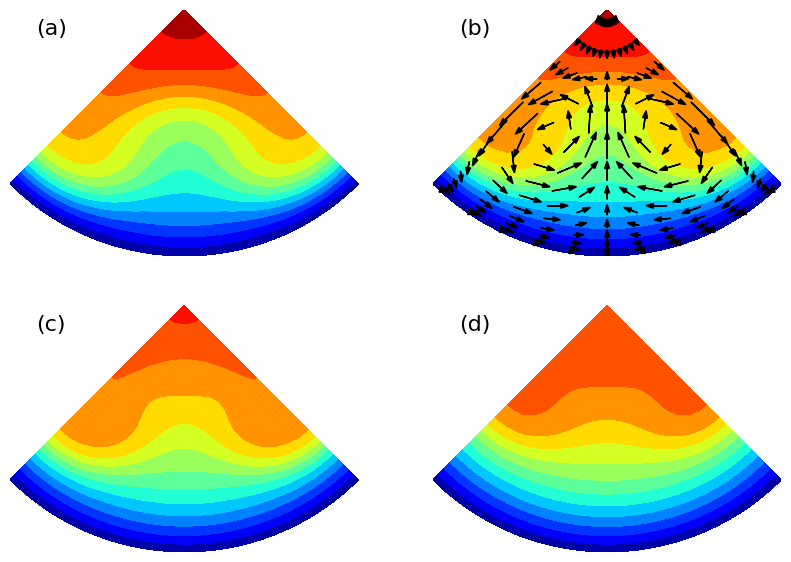
\includegraphics[width=1\linewidth]{VEL_cs.png}}
\caption{Среднее поле скорости $\V$: ряд (a) --- поперечная компонента, ряд~(b)~--- изолинии продольной компоненты. На стенке скорость жидкости равна нулю. Изображено три сечения трубы, $x = 0, 2.5, 5$.}
\label{VEL_cs_pic}
\end{figure}

На рисунке \ref{VEL_cs_pic} приведены поперечная $(V_r, V_\theta)$ и продольная $V_x$ компоненты стационарного течения в области, где пульсации имеют существенную амплитуду. Стационарное поперечное течение соответствует существованию в потоке стационарных продольных вихрей, поддерживающих существование полос. Стационарное поперечное движение направлено от оси трубы к стенке в областях $\theta=k\pi/2$. В этих областях оно переносит быструю жидкость из центра трубы ближе к стенке, создавая тем самым полосы ускорения. При $\theta=\pi/4+k\pi/2$ поперечное движение, напротив, перемещает жидкость от стенки трубы в основной поток. В этих областях образуются полосы замедления. 

Формирующиеся в области небольшой протяженности полосчатые структуры переносятся в переднюю и заднюю часть порыва за счет конвекции. На рисунке \ref{V3D_cs_pic} на линии 1 средняя продольная скорости $V_x$ в системе отсчета, связанной с порывом, равна нулю. В приосевой области, ограниченной этой линией, скорость положительна, а в периферийной отрицательна. Видно, что полосчатые структуры во всех сечениях (кроме переднего, x = 5) располагаются в области отрицательной относительной скорости. Среднее течение с отрицательной скоростью переносит полосчатые структуры в заднюю часть порыва, где они формируют картину, похожую на вытянутые щупальца медузы (смотри рисунок \ref{3D_img}). При $x > 5$ полосчатые структуры концентрируются в приосевой части трубы и конвектируются вперед положительной скоростью относительного движения, благодаря чему в передней части порыва $A_{3D}$ сохраняет заметную величину, несмотря на отсутствие поперечного движения.


\section{Механизм поддержания пульсационной составляющей движения}

\begin{figure}
\center{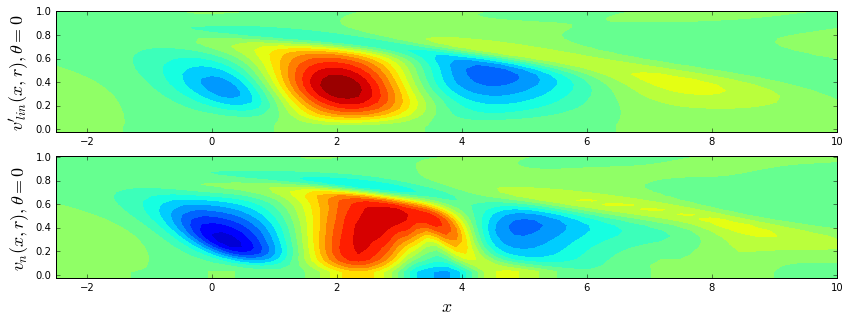
\includegraphics[width=1\linewidth]{lin_ls_cmp.png}}
\caption{Сравнение мгновенного поля продольной скорости пульсаций, возникающих в рамках линеаризованных уравнений \eqref{lin_eq}, $\v'_1$ (a) и пульсационной составляющей движения $\v_n$ (b) в сечении $\theta = 0$. Сплошные изолинии --- положительные значения, прерывистые --- отрицательные.}
\label{lin_ls_cmp_pic}
\end{figure}

Полосчатые структуры достигают максимальной амплитуды в области $x\in[-5,0]$, где создаются условия для возникновения колебаний. Наиболее вероятный механизм генерации колебаний --- механизм потери устойчивости стационарной составляющей течения. Для проверки этой гипотезы стационарное течение $\V$ было исследовано на устойчивость к малым возмущениям $\v'$. Предположение малости $\v'$ позволяет линеаризовать уравнения. Линеаризованные относительно $\v'$ уравнения Навье-Стокса в подвижной системе координат, связанной с порывом, имеют вид:
\begin{equation} \label{lin_eq}
\frac{\partial \v'}{\partial t} = c_m \frac{\partial \v'}{\partial x} - (\V, \nabla) \v' - (\v', \nabla) \V - \nabla p' + \nu \nabla^2 \v'. 
\end{equation}
Здесь $p'$ -- пульсационная составляющая давления. Расход $\v'$ равен нулю. Другие уравнения в постановке задачи линейные и для $\v'$ имеют тот же вид, что и для $\v$. 

Линеаризованные относительно возмущений уравнения с некоторыми случайными начальными условиями интегрировались по времени до выхода решения на режим экспоненциального изменения. Обнаружено, что действительно поле скорости $\V$ неустойчиво к малым возмущениям. Растущее возмущение $\v'_1 \sim e^{(\lambda+i\omega)t}$ имеет инкремент нарастания $\lambda=0.012U/R$ и частоту $\omega=0.116U/R$, близкую к частоте колебаний $2\pi/60R/U=0.105U/R$ в решении на сепаратрисе. Что более существенно, поле скорости растущего решения $\v'_1$ качественно повторяет основные особенности поля скорости пульсационной составляющей движения модельного порыва $\v_n$. В качестве подтверждения на рисунке \ref{lin_ls_cmp_pic} представлены мгновенные поля скорости $\v'_1$ и $\v_n$ в продольном сечении $\theta = 0$. Моменты времени подобраны так, что фазы решений совпадают. Также на рисунке \ref{lin_amp_cmp_pic} для сравнения представлены амплитуды $\v_1'$ и $\v_n$ в нескольких сечениях трубы. Нет сомнений, что колебания возникают в результате линейной неустойчивости стационарной составляющей движения. Решение линейной задачи обладает дополнительной симметрией отражения относительно плоскости $\theta = \pi/4$, выражаемой формулой:
\begin{equation} \label{dop_sym_eq}
(-v_x, -v_r, v_\theta)(x, r, \pi/4 + \theta) = (v_x, v_r, v_\theta)(x, r, \pi/4 - \theta). 
\end{equation} 
В целом, поле $\v'_1$ имеет более простую форму, чем $\v_n$. В частности, $\v'_1$ меняется во времени по гармоническому закону. Воспроизводя основные особенности пульсационной составляющей движения, $\v'_1$ может быть более предпочтительным объектом исследования для объяснения этих особенностей. 

\begin{figure}
\center{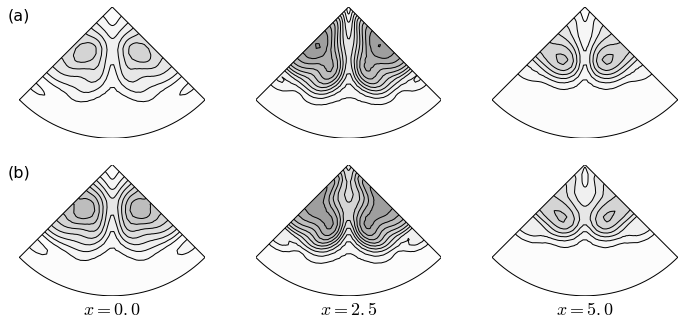
\includegraphics[width=1\linewidth]{lin_amp_cmp.png}}
\caption{Сравнение амплитуды пульсаций, возникающих в рамках линеаризованных уравнений \eqref{lin_eq}, $\v'_1$ --- ряд (a) и пульсационной составляющей движения $\v_n$ --- ряд (b) в нескольких сечения трубы, $x = 0, 2.5, 5$. Вблизи стенки амплитуда пульсаций близка к нулю.}
\label{lin_amp_cmp_pic}
\end{figure}

В реальном течении пульсационная составляющая движения имеет конечную амплитуду и нелинейными слагаемыми в уравнении, описывающем эволюцию пульсаций, уже нельзя пренебрегать. По-видимому, роль нелинейных слагаемых сводится к тому, что они несколько меняют форму пульсаций так, что рост амплитуды пульсационной составляющей движения прекращается. При этом, именно линейные слагаемые определяют форму пульсаций и ответственны за передачу энергии в пульсационную составляющую движения. 

Отметим, что точки максимального роста колебаний находятся на линии $r \approx 0.4$, что соответствует нулевой относительной скорости. По этой причине область порождения колебаний остается неподвижной относительно порыва. Интересно, что в этой же области ($x = 0,\ r \approx 0.4$) происходит смена знака радиальной компоненты осесимметричной составляющей скорости (смотри рисунок~\ref{U2D_pic}(b)). При $x<0$ радиальная скорость положительна, поэтому колебания, возникшие в задней части порыва, относятся в сторону стенки трубы, где относительная скорость отрицательна, и продолжают двигаться вверх по течению. Наоборот, при $x>0$ радиальная скорость направлена к оси трубы. Туда же, в область положительной скорости, сносятся и колебания, обнаруживающиеся в передней части порыва.

Отметим также, что неустойчивость полосчатых структур является неотъемлемой составляющей всех сценариев самоподдержания турбулентности в пристенных течениях. В некоторых работах предполагается, что неустойчивость возникает в пристенных областях полос замедленного движения, где в локальном профиле скорости $V_x(r)$ на фоне наибольшего градиента появляется точка перегиба --- источник неустойчивости в механизме типа Кельвина--Гельмгольца. В частности, именно такой механизм предлагается в качестве механизма возникновения колебаний в турбулентном порыве в \cite{Shimizu2009}. В рассматриваемом нами решении на сепаратрисе это определенно не так. Как видно на рисунке~\ref{puls_cs_pic} в сечении $x=0$, соответствующем максимальной скорости роста колебаний, амплитуда колебаний минимальна как раз в области полосы замедления ($\theta=\pi/4$). Наибольшие колебания развиваются наоборот вблизи полос ускорения, а если быть более точным, в промежуточных областях между полосами. В этих областях стационарная составляющая скорости течения претерпевает наибольшее изменение и имеет точки перегиба, но не как функция радиальной переменной, а как функция угла. Во всех сечениях на рисунке~\ref{puls_cs_pic} сплошными линиями изображены линии нулевой относительной скорости стационарной составляющей течения. Видно, что в сечении $x=0$, где происходит основной рост колебаний, в областях максимальной амплитуды колебаний наблюдается наиболее быстрое изменение скорости как функции угловой переменной.



\section{Влияние продольной неоднородности стационарной составляющей движения на форму пульсаций}

Интересно отметить, что область наибольшей интенсивности пульсаций совпадает с областью резкого изменения скорости на оси трубы (смотри рисунки \ref{ucl_cmp_img}, \ref{amp_pic}). Аналогичную особенность выделяют также в турбулентном порыве \cite{Hof2010}. Для того, чтобы установить влияние продольной неоднородности стационарного течения на образование пульсаций, было исследовано на устойчивость однородное вдоль трубы поле скорости $\U$, воспроизводящее полосчатые структуры. В этом случае коэффициенты в уравнении \eqref{lin_eq} не зависят от $x$, и собственные решения могут быть представлены в виде $\v' = \hat \v(r,\theta,t) e^{i \alpha x}$, что позволяет исключить переменную $x$ из постановки задачи. Уравнение~\eqref{lin_eq} принимает вид
\begin{multline*}
\frac{\partial \hat v_x}{\partial t} = - i \alpha \hat p - i \alpha (U_x - c_f) \hat v_x - (\U_{\perp},\nabla_{\perp}) \hat v_x - 
(\hat \v_{\perp}, \nabla_{\perp}) U_x + \frac{1}{\Re}( \nabla_{\perp}^2 - \alpha^2 ) \hat v_x,
\end{multline*}
\begin{multline*}
\frac{\partial \hat \v_{\perp}}{\partial t} =  - \nabla_{\perp} \hat p - i \alpha (U_x - c_f) \hat \v_{\perp} - (\U_{\perp},\nabla_{\perp}) \hat \v_{\perp} - (\hat \v_{\perp}, \nabla_{\perp}) \U_{\perp} + \frac{1}{\Re}( \nabla_{\perp}^2 - \alpha^2 ) \hat \v_{\perp}, 
\end{multline*}
где знаком $\perp$ обозначена проекция соответствующей величины в плоскость поперечного сечения, ортогональная $x$. Все величины, отмеченные крышечкой, комплексные и не зависят от $x$. В постановке задачи также меняет свой вид уравнение неразрывности:
\begin{equation*}
\nabla_{\perp} \cdot \hat \v_{\perp} = - i \alpha \hat v_x, 
\end{equation*}
и снимается условие периодичности вдоль потока \eqref{bc1_Re}. Задача, таким образом, сводится к двумерной постановке с дополнительным параметром $\alpha$. 

\begin{figure}
\center{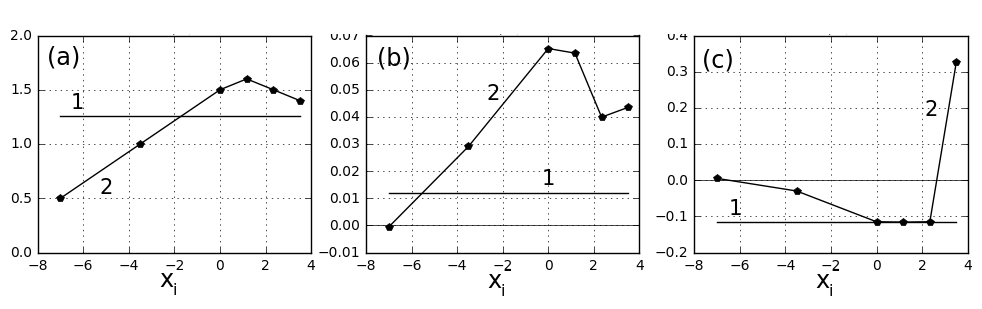
\includegraphics[width=1\linewidth]{cs_lin.png}}
\caption{Значение волнового числа $\alpha$, инкремента нарастания $\lambda$ и угловой частоты $\omega$ (в системе отсчета порыва) для наиболее быстрорастущего собственного возмущения, возникающего на стационарной составляющей движения модельного порыва $\V$ (линия 1) и на однородном вдоль трубы поле скорости, повторяющем $\V$ в сечении с координатой $x$ (линия 2).}
\label{cs_lin_pic}
\end{figure}

На линейную устойчивость исследовано несколько однородных вдоль трубы полей скорости $\U_i$, повторяющих среднее поле скорости модельного порыва $\V$ в одном из поперечных сечений трубы с координатой $x_i$, $\U_i=\V(x_i)$. Все исследованные $\U_i$ в интервале $x_i \in (-8, 4)$ оказались неустойчивы, для каждого из них найдено наиболее неустойчивое собственное возмущение --- собственное возмущение, имеющее наибольшую скорость роста среди всех значений $\alpha$. Наиболее быстро растущее собственное возмущение поля скорости $\U_i$ при фиксированном значении $\alpha$ получено интегрированием произвольного начального возмущения до выхода на экспоненциальный режим роста $\sim e^{(\lambda + i\omega) t}$. 

\begin{figure}
\center{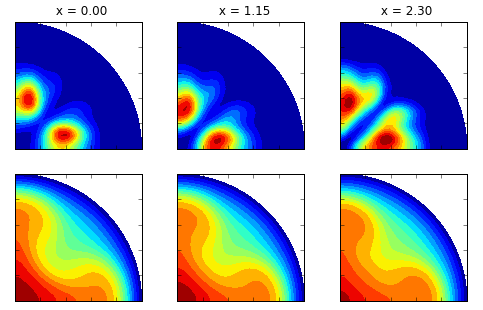
\includegraphics[width=1\linewidth]{cs_lin_map.png}}
\caption{В ряду (a) в поперечном сечении изображена амплитуда пульсаций наиболее быстрорастущего возмущения, возникающего на однородном вдоль трубы поле скорости $\U_i$, приведенном в ряду (b). Однородное поле скорости повторяет среднее поле скорости в сечении $x$, указанном под иллюстрациями.}
\label{cs_lin_map_pic}
\end{figure}

На рисунке \ref{cs_lin_pic} синими точками отмечены полученные значения волнового числа $\alpha$, инкремента нарастания $\lambda$ и угловой частоты $\omega$ для наиболее быстро растущих собственных возмущений поля скорости $\U_i$, как функции $x_i$. Красным представлены соответствующие значения для наиболее быстрорастущего собственного возмущения, возникающего на стационарной составляющей движения модельного порыва $\V$ непосредственно (длина волны и скорость её перемещения оценены примерно). Угловая частота приведена в системе отсчета, связанной с порывом. Наибольшую скорость роста возмущений демонстрируют сечения в диапазоне $x_i \in [0, 2]$. В этой области пульсационная составляющая движения $\v_n$ достигает наибольшей интенсивности (смотри рисунок \ref{amp_pic}). Однако скорость роста возмущений на $\V$ значительно ниже, что может объясняться перераспределением энергии, передаваемой возмущениям в сеченях с координатами $x_i \in [0, 2]$, в те области, где средний профиль скорости имеет более устойчивую форму. Наиболее быстро растущие возмущения поля скорости $\U_i$ при $x_i \in [0,2]$ повторяют форму возмущений, наблюдаемых в модельном порыве. В частности, их волновые числа и угловые частоты близки к соответствующим значениям как для малых возмущений, возникающих на $\V$, так и для пульсационной составляющей движения модельного порыва $\v_n$. Сравнение распределений амплитуды пульсаций в поперечном сечении, возникающих на~$\U_i$ при $x_i \in [0,2]$ (смотри рисунок \ref{cs_lin_map_pic}), и возникающих в модельном порыве (смотри рисунок \ref{lin_amp_cmp_pic}), также демонстрируют качественное соответствие этих решений. Однако уже при $x \approx 3.5$ среднее поле скорости стационарного течения искажается так, что на соответствующем ему $\U_i$ наиболее быстро растущим оказывается возмущение, имеющее качественно другую форму. С этим, в частности, связано резкое отличие значения угловой частоты $\omega$ для этого решения от соответствующих значений, возникающих при меньших $x_i$ (смотри рисунок \ref{cs_lin_pic}). 

Таким образом, может быть сделан вывод о том, что продольная неоднородность стационарной составляющей движения модельного порыва не является определяющим фактором при формировании пульсационной составляющей движения. Возможно, резкое изменение скорости в центральной части трубы является следствием образования пульсаций, по крайней мере, для модельного порыва. 

\section{Механизм образования стационарных продольных вихрей}



\section{Взаимодействие между компонентами движения модельного порыва}

В предыдущих разделах были выделены компоненты движения модельного порыва и основные механизмы взаимодействия между ними. Компоненты движения находятся в динамическом равновесии, поддерживая существование друг друга и, следовательно, самого порыва. Более строго обосновать полученные результаты позволяет анализ баланса кинетической энергии в системе. Вклад каждой из компонент движения в кинетическую энергию других компонент движения может быть непосредственно вычислен, и, в зависимости от его величины, могут быть сделаны выводы о положительном или отрицательном влиянии одной из компонент движения на другую. 

Ниже приведен вывод уравнений баланса кинетической энергии для каждой из компонент движения. 
Осреднение уравнения Навье-Стокса \eqref{NSeq_Re} по времени в системе отсчета, связанной с порывом, дает уравнение баланса импульса стационарной составляющей движения $\V = \overline{\v}^t$:
\begin{equation} \label{VEL_eq}
\pd{\V}{t} =  - \i D - (\V, \nabla) \V - \overline{(\v_n, \nabla) \v_n}^t - \nabla P + \frac{1}{\Re} \nabla^2 \V.
\end{equation}
Здесь и далее большими буквами обозначены средние по времени составляющие соответствующих величин, пульсационную составляющую выделяет нижний индекс $n$. Формально производная по времени от стационарной составляющей движения равна нулю, однако слагаемое $\partial \V/ \partial t$ сохранено в записи уравнения \eqref{VEL_eq}, что упрощает его интерпретацию. В сравнении с уравнением Навье-Стокса, в \eqref{VEL_eq} возникает новое слагаемое $-\overline{(\v_n, \nabla) \v_n}^t$, отвечающее за влияние пульсаций на среднее течение. Его можно рассматривать, как внешнюю силу. 

Последующее осреднение \eqref{VEL_eq} по угловой координате позволяет получить уравнения баланса импульса двумерной компоненты движения $\V_{2D} = \overline{\V}^\theta$:
\begin{multline} \label{V2D_eq}
\pd{\V_{2D}}{t} =  - \i D - (\V_{2D}, \nabla) \V_{2D} - \overline{(\V_{3D}, \nabla) \V_{3D}}^{\theta} - \overline{(\v_n, \nabla) \v_n}^{t,\theta} - \\ - \nabla P_{2D} + \frac{1}{\Re} \nabla^2 \V_{2D}.
\end{multline}
Здесь и далее двумерные компоненты движения обозначены нижним индексом $2D$, индекс $3D$ соответствует трехмерным составляющим. Вычитание \eqref{V2D_eq} из \eqref{VEL_eq} позволяет получить уравнение баланса импульса трехмерной составляющей движения $\V_{3D} = \V - \V_{2D}$:
\begin{multline} \label{V3D_eq}
\pd{\V_{3D}}{t} =  - (\V_{3D}, \nabla) \V_{3D} - (\V_{3D}, \nabla) \V_{2D} - (\V_{2D}, \nabla) \V_{3D} + \\ + \overline{(\V_{3D}, \nabla) \V_{3D}}^{\theta} - \overline{(\v_n, \nabla) \v_n}^{t} + \overline{(\v_n, \nabla) \v_n}^{t, \theta} - \nabla P_{3D} + \frac{1}{\Re} \nabla^2 \V_{3D}.
\end{multline}
Проекция уравнения \eqref{V3D_eq} на направление $x$ дает уравнение, описывающее баланс импульса составляющей движения $\V_S = (V_{x,3D}, 0, 0)$, ассоциированной с полосами повышенной и пониженной скорости. Уравнение баланса импульса составляющей движения $\V_V = (0, V_{r,3D}, V_{\theta,3D})$, воспроизводящей продольные вихри, дает проектирование \eqref{V3D_eq} в поперечную плоскость трубы. Стоит отметить, что $\V_{2D}, \V_{3D}, \v_n$ удовлетворяют условию несжимаемости \eqref{eq0_Re}, в то время как $\V_S$ и $\V_V$ не удовлетворяют ему. 
 

\begin{figure}
\center{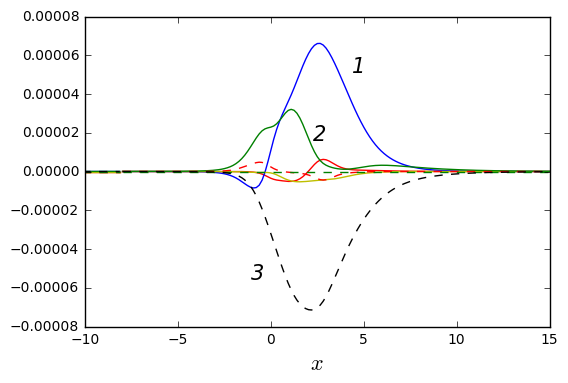
\includegraphics[width=0.6\linewidth]{e1_parts.png}}
\caption{Вклад в кинетическую энергию пульсационной составляющей движения со стороны: 1 --- $\V_S$; 2 --- $\V_{2D}$; 3 --- вязких слагаемых. Другие слагаемые существенного вклада не дают.}
\label{e1_parts_pic}
\end{figure}


Уравнение изменения поля скорости $\v_n = \v - \V$ дает вычитание \eqref{VEL_eq} из \eqref{NSeq_Re}:
\begin{multline} \label{vel1_eq}
\pd{\v_n}{t} = - (\v_n, \nabla) \v_n + \overline{(\v_n, \nabla) \v_n}^t - (\V_{2D}, \nabla) \v_n - (\V_S, \nabla) \v_n - (\V_V, \nabla) \v_n - \\ - (\v_n, \nabla) \V_{2D} - (\v_n, \nabla) \V_S - (\v_n, \nabla) \V_V - \i d_n - \nabla p_n + \frac{1}{\Re} \nabla^2 \v_n. 
\end{multline}
Здесь среднее поле скорости представлено в виде суммы компонент движения $\V = \V_{2D} + \V_S + \V_V$. Они оказывают влияние на пульсационную составляющую движения через соответствующие нелинейные слагаемые. Скалярное умножение каждого слагаемого в \eqref{vel1_eq} на $\v_n$ позволяет получить уравнение изменения кинетической энергии пульсационной составляющей движения. На графике \ref{e1_parts_pic} представлены усреднённые по времени и по сечению трубы вклады каждой из компонент движения и линейных слагаемых в кинетическую энергию пульсаций. Наибольший вклад дает поле скорости $\V_S$, соответствующее полосам повышенной и пониженной скорости, что согласуется с представлениями о возникновении пульсаций вследствие линейной неустойчивости полос. Хотя и не определяющий, но существенный положительный вклад дает базовое течение. Получаемая $\v_n$ энергия расходуется на преодоление вязкого трения. Влияние других слагаемых оказывается незначительно. 

\begin{figure}
\center{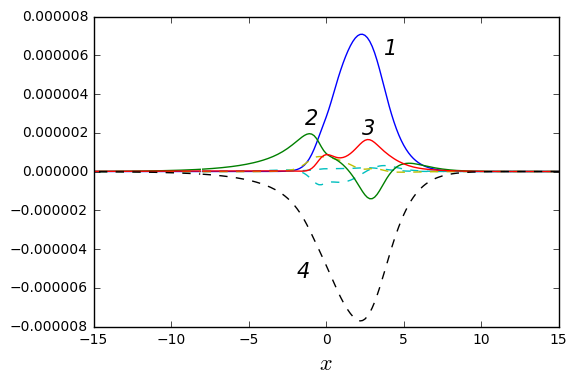
\includegraphics[width=0.6\linewidth]{ev_parts.png}}
\caption{Вклад в кинетическую энергию движения $\V_V$, ассоциированного с продольными вихрями, со стороны: 1 --- $\v_n$; 2 --- $\V_{2D}$; 3 --- градиента давления; 4 --- вязких слагаемых. Другие слагаемые существенного вклада не дают.}
\label{ev_parts_pic}
\end{figure}

Аналогично, скалярное умножение \eqref{V3D_eq} на поле скорости $\V_V$ дает уравнение баланса кинетической энергии движения $\V_V$, ассоциированного с продольными вихрями. Усредненные по сечению трубы вклады каждой из компонент движения и линейных слагаемых в кинетическую энергию $\V_V$ приведены на графике \ref{ev_parts_pic}. В соответствии с общими представлениями, наибольший вклад в продольные вихри дает пульсационная составляющая движения. Также существенный положительный вклад дает внешний градиент давления, однако его величина ниже почти в $5$ раз. Вклад давления отличен от нуля, так как поле скорости $\V_V$ не удовлетворяет условию несжимаемости. В противном случае можно показать, что периодическая составляющая давления обеспечивает лишь перенос энергии, но не её производство. Внешний градиент давления на $\V_V$ влияния не оказывает. Также можно отметить влияние $\V_{2D}$. При $x > 0$ оно отрицательно, а при $x < 0$ --- положительно. Это может быть конвекцией продольной завихренности, формирующейся при положительных $x$, вверх по течению вместе с основным потоком вблизи стенки. Энергия, попадающая в $\V_V$ компенсируется за счет вязкости. 

\begin{figure}
\center{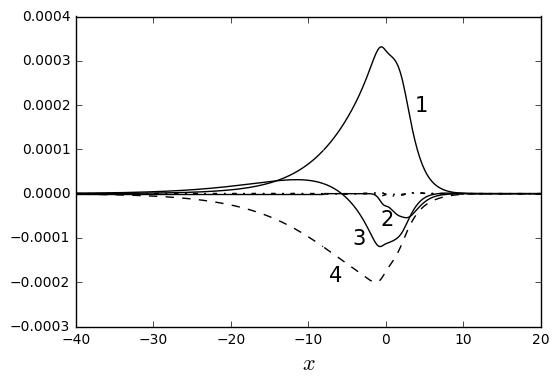
\includegraphics[width=0.6\linewidth]{es_parts.png}}
\caption{Вклад в кинетическую энергию движения $\V_S$, ассоциированного с полосами, со стороны: 1 --- $\V_V$ и $\V_{2D}$; 2 --- $\v_n$; 3 --- $\V_{2D}$; 4 --- вязких слагаемых. Другие слагаемые существенного вклада не дают.}
\label{es_parts_pic}
\end{figure}

Скалярное умножение \eqref{V3D_eq} на поле скорости $\V_S$ дает уравнение баланса кинетической энергии компоненты движения $\V_S$, связанной с полосами повышенной и пониженной скорости. Усредненный по сечению трубы вклад в кинетическую энергию $\V_S$ со стороны различных компонент движения и линейных слагаемых изображен на рисунке \ref{es_parts_pic}. В этом случае наибольший вклад дает слагаемое:
\begin{equation}\label{VS_gen_terms}
\pd{}{t}\frac{\V_S^2}{2} =  - V_{S, x} V_{V, r} \pd{V_{2D, x}}{r} + \dots
\end{equation}
Слагаемое \eqref{VS_gen_terms} выражает совместное влияние $\V_{2D}$ и $\V_V$ на $\V_S$. Это подтверждает представления о возникновении полос вследствие действия <<лифт-ап>> эффекта, в соответствии c которым их формирование происходит за счет действия продольных вихрей на фоне неоднородности продольной скорости, воспроизводимой в данном случае двумерным течением. Пульсации оказывают небольшое отрицательное влияние на формирование полос. Двумерное течение оказывает отрицательное влияние вблизи нуля, в то время, как в задней части порыва, при $x \sim -10$, его влияние оказывается положительным. По-видимому, это связанно с конвективным переносом полос, формирующихся в передней части порыва, в его заднюю часть вблизи стенки, осуществляемым основным течением $\V_{2D}$. Получаемая составляющей движения $\V_S$ энергия расходуется на преодоление вязкого трения.

Полученные в разделе результаты позволяют не только подтвердить уже сложившиеся представления о взаимодействии между различными компонентами движения модельного порыва, но также показать, что все существенные взаимодействия учтены. Приведенные рассуждения опираются на то, что каждая компонента движения представляет только одну особенность течения, и выводы, справедливые для компонент движения, справедливы также и для ассоциированных с ними особенностей течения. Адекватность такого допущения подтверждают результаты, приведенные в предыдущих разделах. 



\section{Выводы по главе}

В главе представлены результаты численного исследования модельного порыва, выполненного автором диссертации. Модельный порыв воспроизводит основные особенности турбулентного порыва, но имеет более простую форму и динамику. Соответствующее модельному порву решение уравнений Навье-Стокса возникает на сепаратрисе, разделяющей области притяжения решений, соответствующих ламинарному и турбулентному режимам течения. Простота временного поведения этого решения позволяет провести его исчерпывающее исследование. 

При изучении модельного порыва установлены его основные характеристики, такие как скорость перемещения вдоль трубы и период его изменения во времени. Составлено представление о внутренней структуре этого решения, в частности, выделены некоторые особенности движения, составляющие цикл его самоподдержания. При изучении модельного порыва наглядно показан процесс образования вытянутых полос, включающий действие <<лифт-ап>> эффекта на ограниченном отрезке длины с последующим конвективным растяжением вдоль стенки трубы. Пульсации в потоке возникают в результате линейной неустойчивости полосчатых структур. Наиболее важный результат проведенного исследования состоит в том, что обнаруженная неустойчивость полосчатого движения противоречит общепринятой точке зрения, согласно которой доминирующей является неустойчивость типа Кельвина--Гельмгольца, возникающая в пристенных областях полос замедленного движения. В рассмотренном примере уровень колебаний в области полос замедления минимален. Генерация колебаний происходит в промежуточной области между полосами на фоне резкого изменения скорости вдоль угловой координаты. По результатам, представленным в главе, может быть сделан ввод о том, что продольные вихри, ответственные за образование полос, формирует пульсационная составляющая движения. Такое представление подтверждается в следующей главе, посвященной механизму образования продольных вихрей.

Полосчатые структуры являются неотъемлемым элементом всех сценариев самоподдержания пристенной турбулентности. Можно ожидать, что выделенный механизм самоподдержания в некоторой степени близок к механизму самоподдержания однородной (нелокализованной) турбулентности в пристенных течениях. Как в однородной турбулентности, так и в локализованных структурах, полосы повышенной и пониженной скорости имеют ограниченную протяженность. Анализ линейной устойчивости однородных вдоль трубы полосчатых структур позволяет сделать вывод о том, что продольная неоднородность существенного влияния на образование пульсационной составляющей движения не оказывает.

Модельный порыв не может быть получен в эксперименте в силу его неустойчивости, что не позволяет выполнить прямое сравнение полученных результатов с экспериментальными данными. Однако согласованность результатов, полученных на нескольких расчетных сетках, между собой и с результатами других авторов позволяет сделать вывод о том, что полученное решение является решением уравнений Навье-Стокса и не зависит от выбора численного метода и параметров расчета. Применимость полученных выводов к турбулентному порыву непосредственно не установлена. Методика такого исследования сегодня не разработана в должной мере. 



